\section{Hardware and Software Mapping}
As figure \ref{fig:Hardware-Software-Mapping} shows, we want to run the \texttt{DriveIT} subsystems on the following hardware:\\

The \texttt{Persistent Storage}, \texttt{DriveIT Web API}, and \texttt{DriveIT Web Client} subsystems will be hosted on a web server running \textit{ASP.NET}. We have chosen \textit{Microsoft Azure} as our host.

The \texttt{DriveIT Web API} uses the \texttt{Persistent Storage} subsystem internally to contact the \textit{Microsoft SQL Server} that runs behind the \textit{Entity Framework}.

The \texttt{DriveIT Web Client} is accessed through a modern web browser using HTTP. The \texttt{DriveIT Web Client} uses the \texttt{DriveIT Web API} internally, and as they are located in the same project, they can be hosted on the same website at \textit{Microsoft Azure}.\\

The \texttt{DriveIT Windows Client} runs on the computers of the used car dealership using the \textit{.NET Framework 4.5}. It furthermore uses the \texttt{CarQuery} subsystem, which helps \texttt{Employee}s fill out missing information about \texttt{Car}s. The \texttt{DriveIT Windows Client} communicates with the \texttt{DriveIT Web API} subsystem through HTTP. The content of the HTTP-requests and responses are \textit{JSON} objects when data transfer is needed.

\begin{figure}[H]
	\centering
	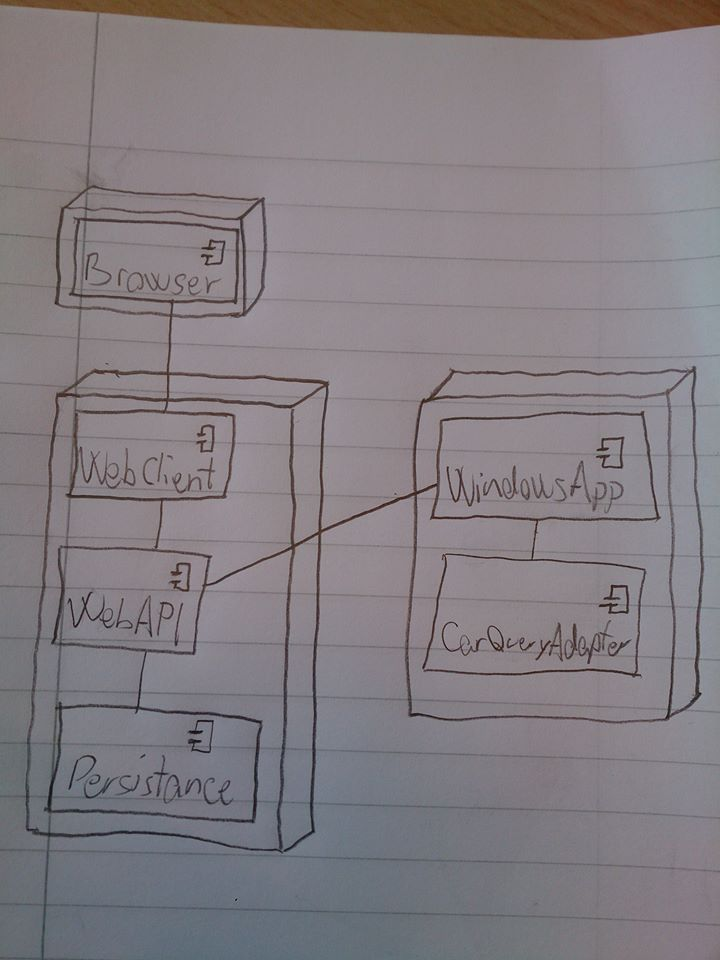
\includegraphics[width=\textwidth]{Figures/HardwareSoftwareMapping}
	\caption{Hardware software mapping of the entire system.}
	\label{fig:Hardware-Software-Mapping}
\end{figure}